% !TEX root = ../main.tex

%先介绍做课题的目的和背景,再引出需要用到COMSOL来进行仿真,再介绍COMSOL


\chapter{绪论}
\section{课题研究背景}
本节简要介绍了分子通信的基本原理与发展现状。
介绍了课题组的微观分子通信实验平台的基本原理,
阐明了了本毕业设计工作的研究内容与研究意义。
\subsection{纳米网络的简述}
随着纳米技术的高速发展,研究者们现在可以
在纳米至微米尺度范围内制造能完成特定功能的结构,
这种微小结构被称为纳米机器(nanomachine)。
由于尺寸较小,单个纳米机器的功能非常有限,只能执行简单的任务
\cite{Weiss_©2003},严重限制了其应用于发展。为了解决这个问题,
纳米机器网络(简称纳米网络,nanonetwork)的概念被提出,
它将多个纳米机器互联、传递信息和彼此协调,扩展了纳米机器在信息采集、运算、储存
等方面的能力,进而使得整个纳米机器群体在更广的覆盖范围内执行更复杂和更精准的任务。
纳米网络在医疗卫生、工业制造、环境治理、国防建设等诸多领域有良好发展前景,
将广泛服务于我们的生产和生活中。

分子通信能够在复杂的生物环境和生物体中实现稳定而且可靠的信息传递,
同时具有生物兼容性好、不受收发器体积和能耗等限制等优点,被认为是组建
纳米网络,尤其是组建面向生物应用的纳米网络,最可行的通信方案之一
\cite{Suda05exploratoryresearch}。
\subsection{分子通信的基本原理}
分子通信(molecular communication)
指的是以生物化学分子作为信息载体的通信技术\cite{Hiyama2010Molecular}。

分子通信作为地球上最古老、最普遍的通信机制之一,广泛存在于自然界。
无论是对简单的单细胞生物,还是对复杂的多细胞动植物来说,分子通信都是维持它们生命必不可少的一环。
例如,许多细菌都会对它们邻居分泌的信号分子(information molecular)做出反应,以协调彼此的行为,并影响它们自身的运动、
产生抗生素、生成孢子等行为,这被成为群体感应。同样的,信号分子(例如信息素)
也广泛的存在于从低等的昆虫到高等的哺乳动物的日常交流中,并深深的影响了它们的行为。
信息素由个体释放,并指导群体里的其他个体前往觅食地,警告同伴有潜在的危险,
以及协调其他各种行为。此外,在多细胞动物体内,细胞与细胞之间也通过信号分子进行通信,
以完成相应的生理功能。例如,我们人体的神经系统中的电信号的传递,就是由神经递质(一种信号分子)
的释放与接收来完成的;在内分泌系统中,内分泌系统会向循环系统释放激素分子,
它作为一种信号分子被远端的目标细胞(靶细胞)所接收,从而完成细胞间的通信,调控靶细胞的行为\cite{Atakan2014Molecular}。

人工分子通信系统基于这一种在自然界就广泛存在的通信方式,
对传统的通信设备进行改造,以生物化学分子作为信息载体
在发射器和接收器之间进行通信。
如图
~\ref{fig:molecular_communication_example}
所示,一个典型的分子通信的典型过程包含三个过程
\cite{基于扩散的分子通信与身体域纳米网络}:
1)发送器(Transmitter)
生成携带着特定编码信息的信息分子(Information Molecule);
2)被释放的信息分子通过流体(液体或气体)介质传送到接又称接收器(Receiver);
3)接收机基于接受到的信息分子的物理或化学特性,对信息进行解码。
\begin{figure}[H]
    \centering
    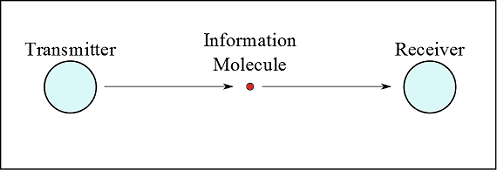
\includegraphics[scale=0.8]{simple model of molecular communication.png}
    \caption{分子通信示意图\cite{compic}}
    \label{fig:molecular_communication_example}
\end{figure}

为方便叙述,本文中“分子通信”特指人工分子通信,而非天然分子通信。

\subsection{分子通信的发展现状与面临挑战}
分子通信这个概念自2005年被提出以来\cite{Suda05exploratoryresearch},
就受到了相关领域研究者的密切关注,发展迅速,
在信道模型与容量分析、调制与解调技术、
信号检测技术、构架和协议设计等方面
已经有多种概念模型和基本框架被建立,
目前已经成为了纳米网络通信机制中非常重要的研究方向。

目前已经有研究成功的
实现了宏观的分子通信实验\cite{10.1007/978-81-322-1007-8_56},这证明了宏观分子通信的可行性。
然而建立纳米网络需要基于微观的分子通信系统,微观分子通信不单单是宏观分子通信
的缩小化,它们之间还存在较大的差别,因此宏观的分子通信实验还不能解决
纳米网络对微观分子通信的实验需求。

总的来说,分子通信的研究主要都集中在理论方面,缺乏实验研究,技术成熟度低。
造成这种现状的最主要的瓶颈问题是
缺少能执行稳定而连续信息传递的微观分子通信平台,使得大量的理论研究
成功无法通过实验进行验证,更进一步阻碍了纳米网络从理论向实际应用的推进,严重
限制了该领域的发展。所以,尽快突破微观分子通信实验平台这个瓶颈问题,已成为纳米网络与分子通信领域
的关注核心和基本共识\cite{Liu1999}。

其中DNA分子通信指的是以DNA为信息分子的分子通信系统。
在当前纳米机器研究中,DNA纳米机器是其中最具有可能迈向第三代
包含人工智能和纳米计算机在内的纳米机器种类\cite{McCutcheon2017}。
因此本课题组正在开展以DNA为信息载体、
以DNA纳米机器为通信主体的微观分子通信实验平台的研究,
为纳米网络提供第一个完整的微观分子通信实验平台,解决本领域瓶颈问题。

\section{课题研究目的及意义}
本毕业设计立足于课题组的现有的DNA分子通信实验平台,对其发送器部分开展理论研究。
我们实现的DNA信息分子的发送器,是一个宏观电信号到微观DNA信号的转化接口。
其主要原理是将锆离子$\ce{Zr^4+}$作为粘合剂胶水,
采用LbL(Layer-by-Layer,逐层)自组装技术在金薄膜表面固定完成多层DNA/$\ce{Zr^4+}$结构。
通过电化学反应执行多层DNA结构的分解与可控释放。
本课题组在先前实验中已经构建完成了基于DNA/$\ce{Zr^{4+}}$LbL自组装结构的
分子通信系统,该系统在外部电压控制下可以将DNA分子从发送机上释放到溶液中。
但对于该分子通信系统的系统模型研究还未开展。

而在所有理论研究中,系统模型是其他理论研究的基础。
首先,虽然目前大量不同的分子通信的理论模型被提出。
但是当前系统模型的研究成果均未经过实验验证其有效性。
更为重要的是,由于DNA的释放与接收机制与以往系统的不同,
因此本项目的DNA微观分子通信的系统模型不同于之前其他
微观分子通信的系统模型。
又由于领域内尚未开展DNA分子通信的研究,
因此需要根据DNA信息分子的释放与接收机制特点,
开展DNA微观分子通信系统模型的研究。

所以本文立足于实验平台,结合DNA微观分子通信特征,开展系统建模的研究。
在课题组实验的基础上,探究DNA受控释放的原理。
综合分子通信理论、电化学反应原理、化学动力学原理、扩散原理
等对DNA的受控释放过程进行建模与仿真。
根据仿真结果对影响该分子通信系统性能的参数进行
研究,并调整参数进行系统的优化。

该研究可以解决目前大量纳米网络与分子通信的理论研究亟需通过实验验证的问题,促
进纳米网络与分子通信的理论研究沿着正确的方向发展。
其次,也将为纳米网络与分子通信从理论研究向实际应用的迈进奠定关键的一步。
因此,无论从理论上还是实践上,本项目的研究都具有重要意义。